\chapter{Socket}

\section{Warum ein Socket?}

Für die Kommunikation zwischen dem Rhaspberry Pi und dem Zug muss eine Schnittstelle bereitgestellt werden, die es erlaubt Anweisungen zu verschicken. Der Pi übermittelt dabei Befehle an den Zug, der Zug muss dem Pi seine Position übermitteln können.
Für diese Schnittstelle ist in diesem Projekt ein Socket zuständig.

\section{Grundfunktionalität}
\label{sec:grundfunktionalität}

Ein Socket ist ein vom Betriebssystem bereitgestelltes Objekt, welches eine Schnittstelle zwischen der Netzwerkprotokoll-Implementierung des Betriebssystems und der Anwendungssoftware bereitstellt. Diese Schnittstelle kann dann zur Kommunikation mit anderen Geräten benutzt werden.\\
Die Socket-API wurde 1983 ursprünglich für BSD-Unix entwickelt, heute ist sie auf jedem POSIX-konformen Betriebssystem, sowie unter Windows verfügbar.\\
Sockets lassen sich grundlegend in zwei Arten unterteilen: Stream Sockets und Datagram Sockets. Stream Sockets benutzen im Regelfall TCP zur Datenübertragung, Datagram Sockets greifen auf UDP zurück.\\
Ein Socket kennt mindestens zwei Teilnehmer, einen Server und mindestens einen Client. \\
Der Server befindet sich zunächst im „listening“-Zustand, bis er eine Anfrage von einem Client erhält. Daraus wird dann ein neuer Server-Socket abgeleitet, welcher sich nach erfolgreichem „accepten“ im „connected“-Zustand befindet. Wird vom Client oder dem Server die Verbindung unterbrochen schließt sich dieser Socket.\\
Zu beachten ist, dass der ursprüngliche Server-Socket erhalten bleibt, sich also bis zum shutdown im „listening“-Zustand befinden wird. So können über die gleiche IP-Adresse und den gleichen Port mehrere Verbindungen parallel entstehen, die Unterscheidung von Mehrfachverbindungen erfolgt durch das Server-Socket und Client-Socket Paar.

\section{Was macht der Socket im Projekt?}

Der Pi öffnet einen Server-Socket, der darauf wartet, dass der Zug dem PI über seine IP und einem festgelegten Port eine Anfrage sendet.\\
Sowohl der Zug als auch der Pi verfügen über mehrere Threads die für die Kommunikation zuständig sind. Ein Klassendiagramm ist in Abbildung \ref{pic:pi_communication} dargestellt.\\

\begin{figure}
	\caption{Beispiel der Kommunikation des Pi}
	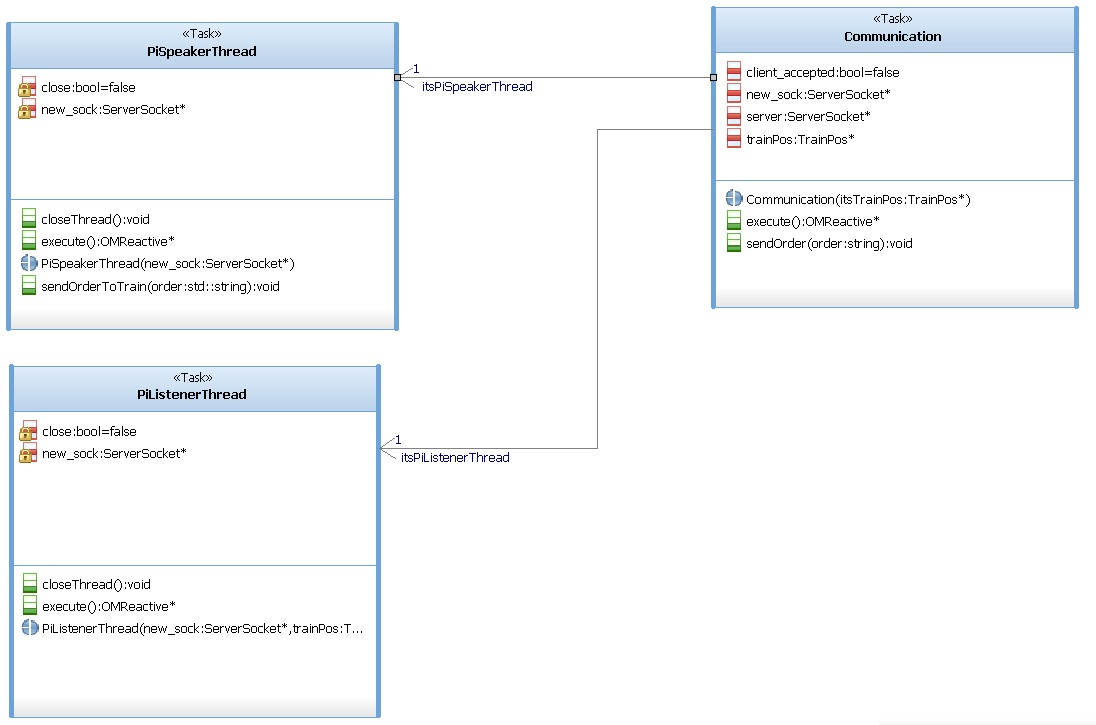
\includegraphics[width=1\textwidth]{content/pictures/socket/pi_speaker_listener.jpg}
	\label{pic:pi_communication}
\end{figure}

\subsection{Implementierung}

\begin{wrapfigure}{rt}{5cm}
	\caption{Socketklasse}
	\centering
	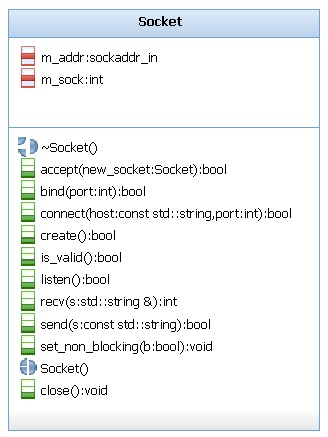
\includegraphics[width=0.3\textwidth]{content/pictures/socket/socket.jpg}
	\label{pic:socket}
\end{wrapfigure}

Als erstes wird eine „Hauptklasse“ Socket (Abbildung \ref{pic:socket}) angelegt, welche eine einfache Implementierung eines C-Sockets bereitstellt.\\
Um die Implementierung weiter zu vereinfachen existieren des weiteren einzelne Klassen für Client- und Server-Socket (Abbildung \ref{pic:server_client}). Diese erben beide von der Hauptklasse und stellen jeweils benötigte Methoden bereit. \\
\begin{figure}
	\caption{Client- und Server-Socketklasse}
	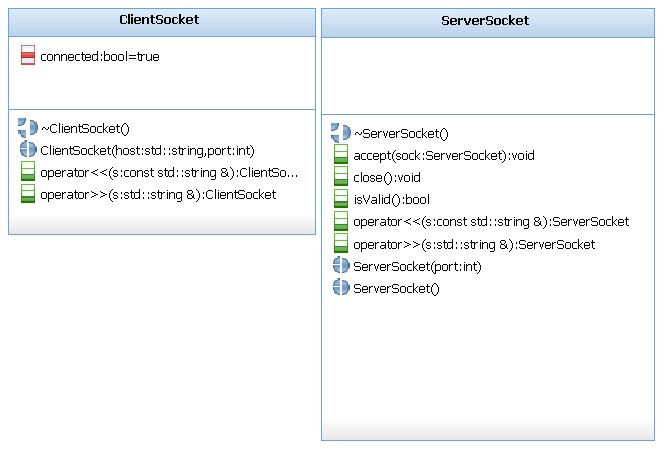
\includegraphics[width=0.8\textwidth]{content/pictures/socket/server_client_socket.jpg}
	\label{pic:server_client}
\end{figure}
Der Thread „Communication“ (Siehe Abbildung \ref{pic:pi_communication}) erzeugt nun einen Socketserver und übergibt diesen nach erfolgreichem Verbinden eines Clients an den „Speaker“ und den „Listener“. Der Aufbau der Kommunikation mit zwei separaten Threads ermöglicht ein gleichzeitiges Lesen und Schreiben.\\
Da es zu keiner Zeit zu einem Verbindungsabbruch kommen darf wird bei jedem neuen Verbindungsversuch eines Clients die alte Verbindung und die beiden Threads „Speaker“ und „Listener“ geschlossen. Anschließend wird die Verbindung neu aufgebaut und neue Threads angelegt. Auf Seite des Clients wird die Information über einen nötigen Neustart der Verbindung direkt im ClientSocket (Abbildung \ref{pic:server_client}, ClientSocket) als Attribut vom Typ bool hinterlegt. Dieses wird in der Kommunikationsklasse des Client ausgelesen und führt gegebenenfalls zum erstellen einer neuen Clientverbindung.\\
Die beiden Operatoren  „<<“ und „>>“ werden für Client- und Socket-Verbindungen überladen um Daten in Form von Strings zu übertragen. Der „Speaker“ bietet hierzu eine Schnittstelle (Auf Pi-Seite „sendOrderToTrain(std::string)“). Der „Listener“ schreibt die gelesenen Daten direkt in einen gemeinsam genutzten Speicherbereich, damit diese auch anderen Threads zur Verfügung stehen.\\
Alle möglichen Fehler innerhalb der Socketklassen werden als Ausnahme der Klasse „SocketException“ geworfen. Diese enthält den Fehlertext und ermöglicht eine Ausgabe des solchen. Die Ausgabe erfolgt in den Kommunikationsklassen von Zug und Pi und wird auf die Konsole geschrieben.





